\let\negmedspace\undefined
\let\negthickspace\undefined
\documentclass[journal,12pt,onecolumn]{IEEEtran}




\usepackage{cite}
\usepackage{amsmath,amssymb,amsfonts,amsthm}
\usepackage{algorithmic}
\usepackage{graphicx}
\usepackage{textcomp}
\usepackage{xcolor}
\usepackage{txfonts}
\usepackage{listings}
\usepackage{enumitem}
\usepackage{mathtools}
\usepackage{gensymb}
\usepackage[breaklinks=true]{hyperref}
\usepackage{tkz-euclide} % loads  TikZ and tkz-base
\usepackage{listings}
\usepackage{circuitikz}
\usepackage{graphicx}

%\newcounter{MYtempeqncnt}
\DeclareMathOperator*{\Res}{Res}
%\renewcommand{\baselinestretch}{2}
\renewcommand\thesection{\arabic{section}}
\renewcommand\thesubsection{\thesection.\arabic{subsection}}
\renewcommand\thesubsubsection{\thesubsection.\arabic{subsubsection}}

\renewcommand\thesectiondis{\arabic{section}}
\renewcommand\thesubsectiondis{\thesectiondis.\arabic{subsection}}
\renewcommand\thesubsubsectiondis{\thesubsectiondis.\arabic{subsubsection}}

% correct bad hyphenation here
\hyphenation{op-tical net-works semi-conduc-tor}
\def\inputGnumericTable{}                                 %%

\lstset{
	frame=single,
	breaklines=true,
	columns=fullflexible
}

\newtheorem{theorem}{Theorem}[section]
\newtheorem{problem}{Problem}
\newtheorem{proposition}{Proposition}[section]
\newtheorem{lemma}{Lemma}[section]
\newtheorem{corollary}[theorem]{Corollary}
\newtheorem{example}{Example}[section]
\newtheorem{definition}[problem]{Definition}
\newcommand{\BEQA}{\begin{eqnarray}}
	\newcommand{\EEQA}{\end{eqnarray}}
\newcommand{\define}{\stackrel{\triangle}{=}}
\newcommand\figref{Fig.~\ref}
\newcommand\tabref{Table~\ref}
\bibliographystyle{IEEEtran}
%\bibliographystyle{ieeetr}


\providecommand{\mbf}{\mathbf}
\providecommand{\pr}[1]{\ensuremath{\Pr\left(#1\right)}}
\providecommand{\qfunc}[1]{\ensuremath{Q\left(#1\right)}}
\providecommand{\sbrak}[1]{\ensuremath{{}\left[#1\right]}}
\providecommand{\lsbrak}[1]{\ensuremath{{}\left[#1\right.}}
\providecommand{\rsbrak}[1]{\ensuremath{{}\left.#1\right]}}
\providecommand{\brak}[1]{\ensuremath{\left(#1\right)}}
\providecommand{\lbrak}[1]{\ensuremath{\left(#1\right.}}
\providecommand{\rbrak}[1]{\ensuremath{\left.#1\right)}}
\providecommand{\cbrak}[1]{\ensuremath{\left\{#1\right\}}}
\providecommand{\lcbrak}[1]{\ensuremath{\left\{#1\right.}}
\providecommand{\rcbrak}[1]{\ensuremath{\left.#1\right\}}}
\theoremstyle{remark}
\newtheorem{rem}{Remark}
\newcommand{\sgn}{\mathop{\mathrm{sgn}}}
\providecommand{\abs}[1]{\left\vert#1\right\vert}
\providecommand{\res}[1]{\Res\displaylimits_{#1}}
\providecommand{\norm}[1]{\left\lVert#1\right\rVert}
%\providecommand{\norm}[1]{\lVert#1\rVert}
\providecommand{\mtx}[1]{\mathbf{#1}}
\providecommand{\mean}[1]{E\left[ #1 \right]}
\providecommand{\fourier}{\overset{\mathcal{F}}{ \rightleftharpoons}}
%\providecommand{\hilbert}{\overset{\mathcal{H}}{ \rightleftharpoons}}
\providecommand{\system}{\overset{\mathcal{H}}{ \longleftrightarrow}}
%\newcommand{\solution}[2]{\textbf{Solution:}{#1}}
\newcommand{\solution}{\noindent \textbf{Solution: }}
\newcommand{\cosec}{\,\text{cosec}\,}
\providecommand{\dec}[2]{\ensuremath{\overset{#1}{\underset{#2}{\gtrless}}}}
\newcommand{\myvec}[1]{\ensuremath{\begin{pmatrix}#1\end{pmatrix}}}
\newcommand{\mydet}[1]{\ensuremath{\begin{vmatrix}#1\end{vmatrix}}}
\renewcommand{\abstractname}{Question}


\let\vec\mathbf

\vspace{3cm}


\newcommand{\permcomb}[4][0mu]{{{}^{#3}\mkern#1#2_{#4}}}
\newcommand{\comb}[1][-1mu]{\permcomb[#1]{C}}

%\IEEEpeerreviewmaketitle

\newcommand \tab [1][1cm]{\hspace*{#1}}
%\newcommand{\Var}{$\sigma ^2$}
\usepackage{amssymb}
\usepackage{amsmath}
\title{
	
	\title{NCERT Maths 11.9.2 Q9}
	\author{EE23BTECH11014- DEVARAKONDA GUNA VAISHNAVI$^{*}$% <-this % stops a space
	}
	
	
}
\begin{document}
\maketitle
	
\textbf{Question:} 
The sum of the first $n$ terms of two arithmetic progressions (AP) is in the ratio $5n+4 : 9n+6$. Find the ratio of their 18th terms.

\solution:

\begin{table}[htbp]
	\centering
    \begin{tabular}{|c|c|c|}
    \hline
    \textbf{Parameter} &\textbf{value}& \textbf{Description} \\
    \hline
    \( x_1(0) \) & $\frac{9}{2}$& First term of the first arithmetic progression (AP). \\
    \hline
    \( x_2(0) \) &$\frac{15}{2}$& First term of the second arithmetic progression (AP).  \\
    \hline
    \( d_1 \) & 5 &Common difference of the first AP. \\
    \hline
    \( d_2 \) & 9&Common difference of the second AP. \\
    \hline
    \( n \) & - &Index of the term in the sequences. \\
    \hline
    \end{tabular}
    \label{tab:parameters}
     \caption{Input Parameters}
\end{table}

\begin{align}
x_1(n)=(x_1(0)+nd_1)u(n)
\label{eq:1}
\end{align}
\begin{align}
x_2(n)=(x_2(0)+nd_2)u(n)
\label{eq:2}
\end{align}
\begin{align}
\frac{y_1(n)}{y_2(n)}=\frac{\frac{n}{2}\left[ 2x_1(0) +(n-1)d_1 \right]}{\frac{n}{2}\left[ 2x_2(0) +(n-1)d_2 \right]}&= \frac{5n+4}{9n+6}\\
\frac{2x_1(0) +nd_1-d_1}{2x_2(0) +nd_2-d_2 }&= \frac{5n+4}{9n+6}
\end{align}
\begin{center}
On comparing we get, $ d_1 = 5 $ and $ d_2 = 9$ \\
\end{center}
\begin{align}
2x_1(0) - d_1 &= 4\\
x_1(0) &=\frac{9}{2}
\end{align}
\begin{align}
2x_2(0)- d_2&=6\\
x_2(0) &=\frac{15}{2}
\end{align}
Refer equation\eqref{eq:uz}  and equation\eqref{eq:uzder}from appendix
\begin{align}
   \implies X_1(z^{-1}) &=\frac{9/2}{1-z^{-1}} + \frac{ 5z^{-1}}{(1-z^{-1})^2}\\
    \implies X_2(z^{-1})&= \frac{15/2}{1-z^{-1}} + \frac{9z^{-1}}{(1-z^{-1})^2}
\end{align}
\begin{align}
x_1(n)&= \lbrace 9/2,19/2,29/2,...\rbrace 
\end{align}
\begin{align}
x_2(n)&= \lbrace 15/2,33/2,51/2,...\rbrace 
\end{align}
\begin{align}
\implies \frac{x_1(18)}{x_2(18)}=\frac{179}{321}
\end{align}
\begin{figure}[h!]
	\centering
	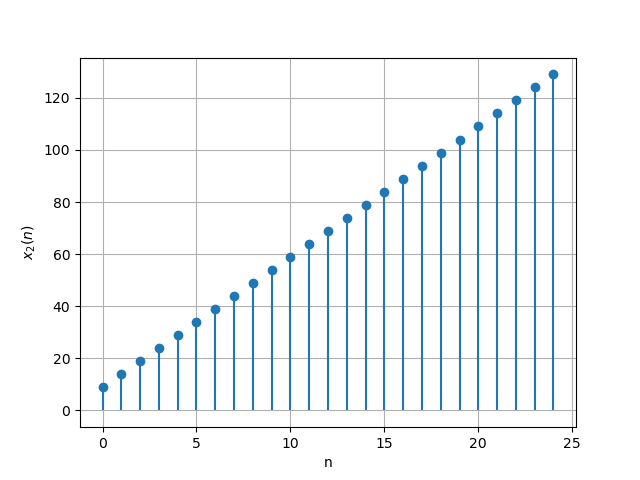
\includegraphics[width=\columnwidth]{figs/fig1.png}
	\label{fig:plot}
	\caption{\large{stem plot of $x_1(n)$}}
\end{figure}
\begin{figure}[h!]
	\centering
	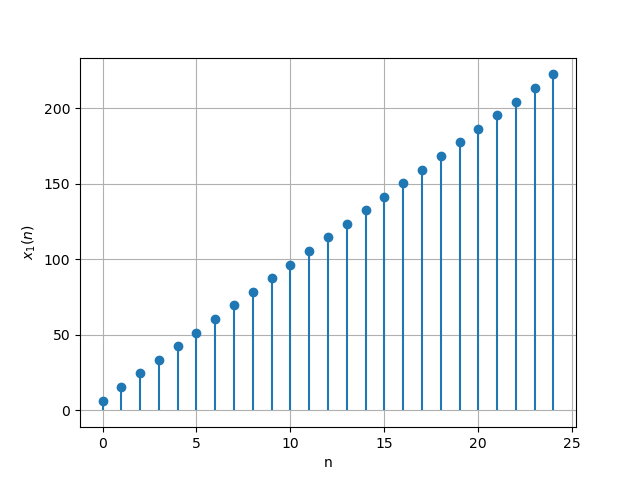
\includegraphics[width=\columnwidth]{figs/fig2.png}
	\label{fig:plot}
	\caption{\large{stem plot of $x_2(n)$}}
\end{figure}
\end{document}
